% ===========================================================
% 5. BENCHMARK
% ===========================================================
\section{Benchmark}
\label{sec:benchmark}

Existing navigation benchmarks fall short of evaluating two
capabilities that are central to deployable real-world agents:
(i) closed-loop, social-rule-aware navigation in heterogeneous
indoor and outdoor environments, and
(ii) final-meters arrival at the physical entrance of a named
point of interest in dense commercial streetscapes. We therefore
introduce two complementary benchmarks built on the same
high-fidelity 3DGS reconstruction stack: \textbf{ABotN-PointBench}
for coordinate-conditioned navigation and \textbf{ABotN-POIBench} for
name-conditioned POI navigation. Figure~\ref{fig:benchmarks} gives
an overview of both benchmarks and the unified scene construction
pipeline shared by them. Then we describe the ABotN-PointBench and ABotN-POIBench in
detail, respectively.

\begin{figure*}[t]
\centering
% 
\includegraphics[width=\linewidth]{benchmarks.pdf}
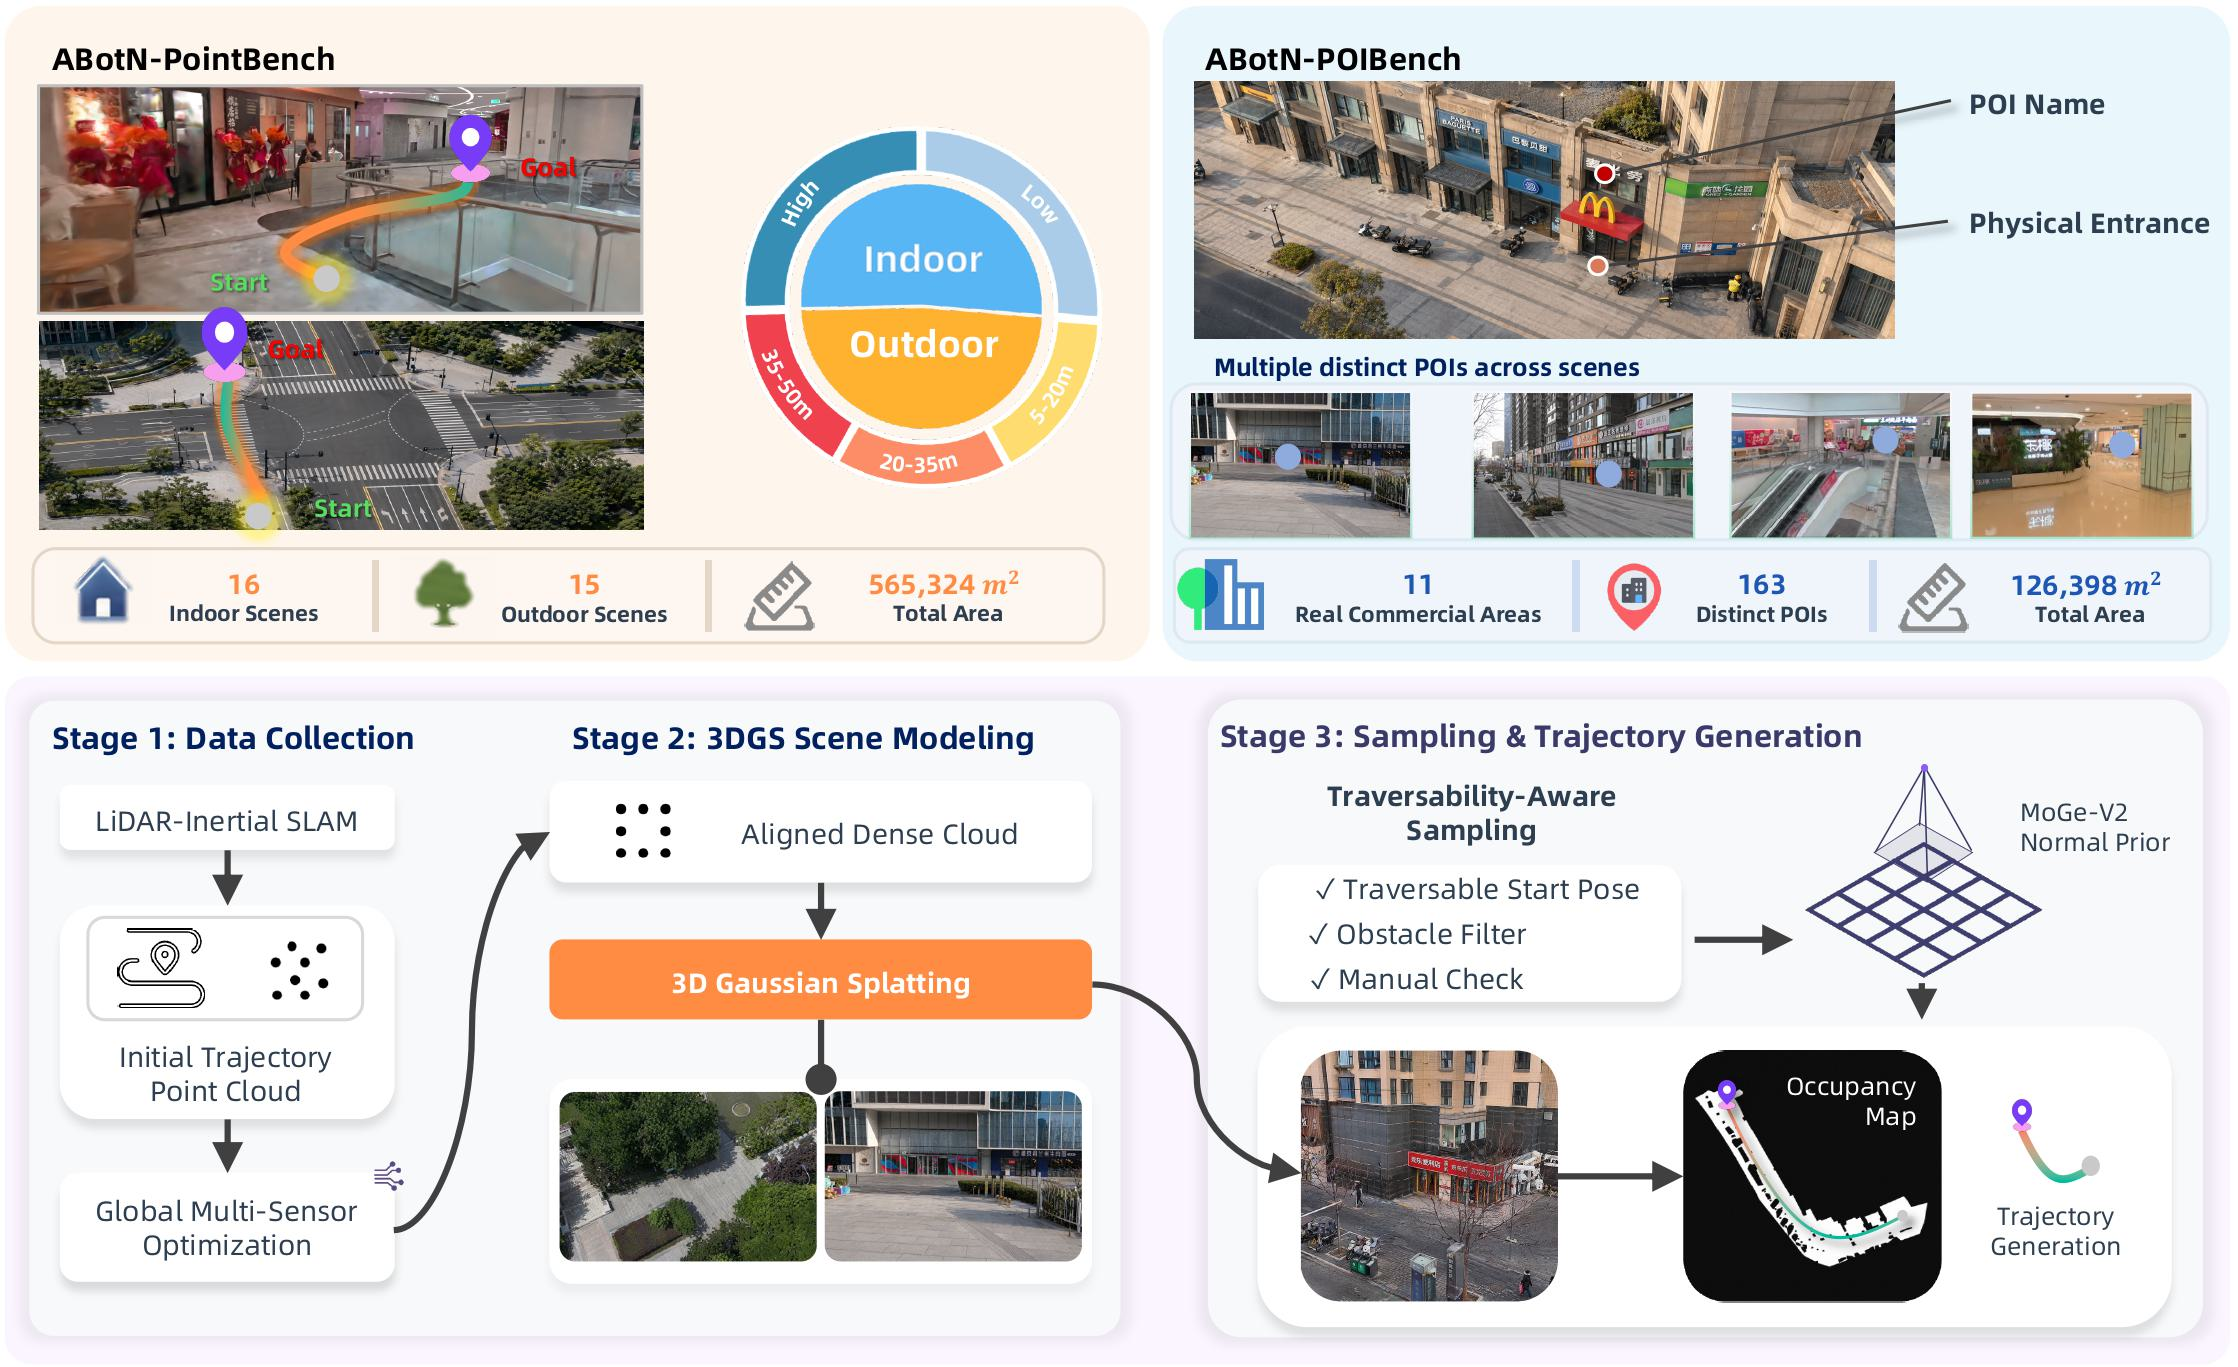
\includegraphics[width=\linewidth]{figs_jpg/benchmarks.jpg}

\caption{\textbf{Overview of the ABotN Benchmark Suites and their
Unified Scene Construction Pipeline.} Top: Dataset
statistics and hierarchical distance splits for \textbf{ABotN-PointBench}
(left) and
\textbf{ABotN-POIBench} (right). Bottom: The unified three-stage generation
pipeline: (1) high-fidelity data collection via LiDAR-inertial
SLAM; (2) photorealistic 3DGS scene modeling initialized by
aligned dense point clouds; and (3) traversability-aware query
sampling and ground-truth reference trajectory generation using
A$^{\!*}$ on MoGe-V2-derived 2D occupancy grids.}
\label{fig:benchmarks}
\end{figure*}

\subsection{ABotN-PointBench}
\label{sec:bench-pointgoal}

\paragraph{Motivation.}
Most prior \textit{point-goal} benchmarks suffer from three structural
gaps. \emph{Scene homogeneity}: representative works such as
CityWalker evaluate exclusively on street blocks, leaving malls,
parks, and indoor commute settings unmeasured. \emph{Open-loop
protocol}: single-step waypoint regression decouples prediction
from downstream control and ignores compounding errors that
dominate real deployment. \emph{Social rules ignored}: traditional
benchmarks score only geometric arrival, so policies that cut
across vehicle lanes or trample lawns are rewarded equally with
socially compliant ones. ABotN-PointBench is the first
closed-loop, high-fidelity benchmark that explicitly addresses all
three gaps for indoor and outdoor \textit{point-goal} navigation.

\paragraph{Scene Construction.}
We collect 31 real-world scenes (16 indoor, 15 outdoor) spanning
shopping malls, parks, road intersections, and daily commute
corridors, and reconstruct each as a high-fidelity 3DGS
environment. Annotators then label every scene with a
fine-grained walkability map that distinguishes legally
traversable regions (sidewalks, crosswalks, building entrances,
intersection paths) from violating regions (vehicle and
non-motorized lanes, lawns, static obstacles such as bicycles,
pillars, and flower beds). The
resulting occupancy maps double as ground truth for both episode
generation and compliance scoring.

\paragraph{Episode and Reference-Trajectory Generation.}
For every scene we run A$^{\!*}$ on the annotated occupancy map to
produce shortest feasible paths used as reference trajectories for
efficiency metrics (e.g., SPL), yielding 465 distinct reference
trajectories.
% across over 59K frames. 
Targets are stratified by distance
to cover both short-horizon precision and long-horizon endurance:
indoor targets are sampled in $3$--$20$\,m, while outdoor targets
are partitioned into three buckets ($5$--$20$, $20$--$35$,
$35$--$50$\,m). Each episode is rolled out closed-loop in our
in-house 3DGS evaluator, with the agent receiving real-time RGB
and a global coordinate.

\paragraph{Difficulty Stratification.}
To probe robustness under increasing navigational demands, episodes
are stratified by path length.
\emph{Outdoor} (15~scenes, 5 episodes per scene per tier):
Low ($5$--$20$\,m), Medium ($20$--$35$\,m), High ($35$--$50$\,m),
yielding 75 episodes per tier. Because the large-scale outdoor
occupancy annotations inevitably carry slight boundary deviations,
the outdoor split adopts a relaxed collision budget---an episode is
counted as successful only if the agent arrives with fewer than three
collision events; we denote this metric SR$_{<3\text{col}}$. This
redundant tolerance prevents minor labeling inaccuracies near
obstacle boundaries from being misinterpreted as genuine navigation
failures.
\emph{Indoor} (16~scenes, 8~Low-difficulty + 8~High-difficulty):
targets range over $3$--$20$\,m.  Additionally, since indoor scenes
are compact and precisely annotated, indoor episodes
impose a strict collision budget---an episode is counted as
successful only if the agent arrives with no collision
event; we denote this metric SR$_{<1\text{col}}$.

\paragraph{Metrics.}
We report the following metrics:
\begin{itemize}[nosep,leftmargin=1.2em]
\item \textbf{SR} (Success Rate): fraction of episodes where the
  agent reaches within a threshold distance of the target under the
  split-specific collision budget (SR$_{<3\text{col}}$ outdoors,
  SR$_{<1\text{col}}$ indoors).
\item \textbf{SPL} (Success weighted by Path Length): SR discounted
  by path efficiency relative to the A$^{\!*}$ reference trajectory.
% \item \textbf{DCR} (Distance Compliance Rate): for a successful
%   trajectory, DCR$=d_{\text{compliant}}/d_{\text{actual}}$, i.e., the
%   fraction of traversed distance that lies inside socially
%   compliant regions (sidewalks, crosswalks, building entrances,
%   etc.).  For a failed episode, DCR$=0$.  We report the average
%   over all $N$ episodes:
%   \[
%   \text{DCR}_{\text{avg}} = \frac{1}{N}\sum_{i=1}^{N}\text{DCR}_i.
%   \]
% \item \textbf{TCR} (Time Compliance Rate): analogous to DCR but
%   measures the fraction of \emph{time} the agent spends inside
%   compliant regions.  For a successful trajectory,
%   TCR$=t_{\text{compliant}}/t_{\text{actual}}$; for a failed
%   episode, TCR$=0$, averaged identically:
%   \[
%   \text{TCR}_{\text{avg}} = \frac{1}{N}\sum_{i=1}^{N}\text{TCR}_i.
%   \]
\end{itemize}

% DCR and TCR jointly penalize policies that succeed geometrically
% but violate social rules en route or at the goal.  Because failed
% episodes receive a score of zero, both metrics inherently
% correlate with task success, making them comprehensive measures
% of ``reach the goal \emph{and} obey the rules.''


\subsection{ABotN-POIBench}
\label{sec:bench-poigoal}

\paragraph{Motivation.}
\textit{POI-goal} navigation requires the agent to reach the
\emph{physical entrance} of a named POI, not merely an abstract
coordinate or a coarse semantic region. Existing protocols sit at
two unsatisfactory extremes: open-loop benchmarks like BridgeNav
evaluate only single-step waypoint prediction and cannot reflect
closed-loop interaction, while coarse-grained benchmarks like
CitySeeker evaluate only at the block or graph-node level and
miss the entrance-level final-meters arrival accuracy that real
deployment demands. ABotN-POIBench is, to our knowledge, the first
closed-loop, high-fidelity benchmark for real-world \textit{POI-goal}
navigation.

\paragraph{Scene Construction.}
We select 11 real commercial regions with high POI density and
diverse storefront types. Sidewalk width is treated as a hard
constraint during selection: robots have limited camera
heights and vertical FOV, so excessively narrow streets
would make high-mounted signage invisible from the agent's
perspective. Each region is reconstructed as a 3DGS scene through
a four-stage pipeline: (i) LiDAR-Inertial SLAM yields an initial
trajectory and point cloud; (ii) global multi-sensor optimization
jointly refines camera poses and produces a dense LiDAR point
cloud aligned with the captured RGB frames; (iii) the dense
LiDAR points directly initialize the 3D Gaussians, which are then
optimized against the RGB observations and refined camera poses
for improved geometric consistency, sharply improving
reconstruction quality on textureless street surfaces; (iv) a
dense triangle mesh is extracted from the optimized Gaussians and
registered with our in-house 3DGS evaluator as collision
geometry, ensuring both photorealistic fidelity and physically
faithful interaction.

\paragraph{POI and Entrance Annotation.}
The benchmark covers 11 commercial regions totaling
$\sim$126{,}398\,m$^2$, 163 distinct POIs, $>$38\,M Gaussian
points, $\sim$2.81\,M mesh vertices, and $\sim$4.40\,M mesh faces.
Each POI is annotated with both its name and its physical
entrance: the entrance is represented as a ground-flush horizontal
bounding frame defined by two ground-aligned points that span the
doorway width. This entrance frame serves as the ground-truth
arrival region against which final-meters success is judged,
avoiding the ambiguity of a single arrival coordinate.

\paragraph{Start Sampling and Reference Trajectories.}
For every annotated POI, we sample multiple starting poses within a
radius around the entrance under traversability-aware constraints:
(i) start point must lie inside human-annotated walkable regions;
(ii) grass, steps, and large obstacles unsuited to quadruped
locomotion are excluded; (iii) every start point is manually checked to
guarantee that, from the low viewpoint, at least
partial signage of the target POI is visible. To enable efficiency
metrics, we generate ground-truth reference trajectories by
estimating surface normals with MoGe-V2, classifying upward-facing
surfaces as traversable ground and walls/pillars as obstacles,
projecting to a 2D top-down occupancy grid, and running A$^{\!*}$
from the start to the entrance frame.

\paragraph{Metrics.}
We report success rate at a $2$\,m entrance threshold (SR$_{<2\mathrm{m}}$)
and SPL against the A$^{\!*}$ reference. The strict
entrance-distance criterion enforces final-meters arrival accuracy
and prevents trivial credit for stopping in the rough vicinity of
the storefront.
